% $Id: template.tex 11 2007-04-03 22:25:53Z jpeltier $

\documentclass{vgtc}                          % final (conference style)
%\documentclass[review]{vgtc}                 % review
%\documentclass[widereview]{vgtc}             % wide-spaced review
%\documentclass[preprint]{vgtc}               % preprint
%\documentclass[electronic]{vgtc}             % electronic version

%% Uncomment one of the lines above depending on where your paper is
%% in the conference process. ``review'' and ``widereview'' are for review
%% submission, ``preprint'' is for pre-publication, and the final version
%% doesn't use a specific qualifier. Further, ``electronic'' includes
%% hyperreferences for more convenient online viewing.

%% Please use one of the ``review'' options in combination with the
%% assigned online id (see below) ONLY if your paper uses a double blind
%% review process. Some conferences, like IEEE Vis and InfoVis, have NOT
%% in the past.

%% Figures should be in CMYK or Grey scale format, otherwise, colour
%% shifting may occur during the printing process.

%% These three lines bring in essential packages: ``mathptmx'' for Type 1
%% typefaces, ``graphicx'' for inclusion of EPS figures. and ``times''
%% for proper handling of the times font family.

\usepackage{mathptmx}
\usepackage{graphicx}
\usepackage{times}

\usepackage{algorithm}% http://ctan.org/pkg/algorithm
\usepackage{algpseudocode}% http://ctan.org/pkg/algorithmicx

\usepackage{url}

\usepackage{color}
\newcommand{\m}{\textcolor{black}}

\usepackage{multirow}
\usepackage{tabularx}

\newcommand*{\WineMenuColor}{black}%
\newcommand*{\StartMenu}{\includegraphics[scale=0.2]{img/object_label.png}}%
\newcommand*{\WinMenu}[1]{
\StartMenu}

%\textcolor{red/blue/green/black/white/cyan/magenta/yellow}{text}

\usepackage{algpseudocode}


\algnewcommand{\IIf}[1]{\State\algorithmicif\ #1\ \algorithmicthen}
\algnewcommand{\EndIIf}{\unskip\ \algorithmicend\ \algorithmicif}

%\usepackage[demo]{graphicx}

%% We encourage the use of mathptmx for consistent usage of times font
%% throughout the proceedings. However, if you encounter conflicts
%% with other math-related packages, you may want to disable it.

%% If you are submitting a paper to a conference for review with a double
%% blind reviewing process, please replace the value ``0'' below with your
%% OnlineID. Otherwise, you may safely leave it at ``0''.
%\onlineid{2707}

%% declare the category of your paper, only shown in review mode
\vgtccategory{Research}

%% allow for this line if you want the electronic option to work properly
\vgtcinsertpkg

%% In preprint mode you may define your own headline.
%\preprinttext{To appear in an IEEE VGTC sponsored conference.}

%% Paper title.

\title{Unfolding the City: Exploring Mobility Patterns with Individual Characteristics}
%Interaction-On: Interaction Argument to Facilitate Visual Exploration on Web
%Filter+: Interaction Argument for Existing Web-based Visualizations

%% This is how authors are specified in the conference style

%% Author and Affiliation (single author).
%%\author{Roy G. Biv\thanks{e-mail: roy.g.biv@aol.com}}
%%\affiliation{\scriptsize Allied Widgets Research}

%% Author and Affiliation (multiple authors with single affiliations).
%\author{Min Lu\thanks{e-mail: min.lu@pku.edu.cn} %
%\and Jie Liang\thanks{e-mail: christy.jie@gmail.com} %
%\and Zhang Yu\thanks{e-mail: yuzhang94@pku.edu.cn}
%\and Guozheng Li\thanks{e-mail: liguozhengsdu@gmail.com}
%\and Siming Chen\thanks{e-mail: simingchen3@gmail.com}
%\and Zongru Li\thanks{e-mail: zongru.li@pku.edu.cn}
%\and Xiaoru Yuan\thanks{e-mail: xiaoru.yuan@pku.edu.cn}
%\affiliation{\scriptsize  \\ Peking University}}

% \author{Min Lu\textsuperscript{1}\thanks{e-mail: min.lu@pku.edu.cn}\\ %
% \and Jie Liang\textsuperscript{2}\thanks{e-mail: jie.liang@uts.edu.au}\\ %
% \and Yu Zhang\textsuperscript{1}\thanks{e-mail: yuzhang94@pku.edu.cn}\\ %
% \and Guozheng Li\textsuperscript{1}\thanks{e-mail: guozheng.li@pku.edu.cn}\\ %
% \and Siming Chen\textsuperscript{1}\thanks{e-mail: siming.chen@pku.edu.cn}\\ %
% \and Zongru Li\textsuperscript{1}\thanks{e-mail: zongru.li@pku.edu.cn}\\%
% \and Xiaoru Yuan\textsuperscript{13}\thanks{e-mail: xiaoru.yuan@pku.edu.cn}%
% }
% \affiliation{\scriptsize 1) Key Laboratory of Machine Perception (Ministry of Education), and School of EECS, Peking University, China  \\ 2) School of Engineer and Information Technology, The University of
% Technology, Sydney, Australia \\3) Beijing Engineering Research Center of Virtual Simulation and
% Visualization, China}

%% Author and Affiliation (multiple authors with multiple affiliations)
%\author{}

%% A teaser figure can be included as follows, but is not recommended since
%% the space is now taken up by a full width abstract.
\teaser{
  \includegraphics[width= .95\linewidth]{pictures/teaser.eps}
  \caption{Interface: \m{XXX...}}
  \label{fig:teaser}
  %\footnotetext{http://developer.android.com/guide/basics/what-is-android.html}
}

%\cite{papervis}

%% Abstract section.

\abstract{A city is shaped not only by its assembled infrastructures but also the population living inside it. Population in a wide range of individual characteristics visit places with different weights and preferences, sculpturing the city into a space of diverse mobility patterns. Different from the well study of anonymous travel behaviours, the mobility patterns of characterized individuals, is less studied because of the challenges in collection and analysis of data with privacy. In this work, we take a step forward and carefully perform an online census to collect individual profiles and movements from large-scale volunteers. Then we develop a visual analytic system to investigate the mobility patterns of groups by specifying characteristics. To facilitate the identification of characterized groups, individuals are embedded in t-SNE projection for abstract overview as well as drawn as vivid graphics by a data-driven profile method for detail examination. A 2.5D spatial visualization is proposed to maintain a compact multivariable analysis by relaxing the z-axis to encode information incorporating visiting frequency, demands, traveling distance, etc. Together with the cross-filter and flexible 2.5D interactions, the effectiveness and usability of the system is well demonstrated by a study made in Shenzhen.}

%added on a wide range of online visualizations.

%Different from toolkits that integrate interactions during the visualization construction, \textit{interaction-On} provides interactions for the visualizations that has been produced.

%Instead of integrating interactions into the visualization pipeline \textit{Interaction-On} takes the

%Different from interaction toolkits used by visualization producers, \textit{Interaction-On} serves as the toolkits used by visualization consumers.

%Rather than integrating interactions into the visualization pipeline, \textit{Interaction-On} Taking a visualization as input, \textit{Interaction-On} extracts objects and attributes, provides a set of interactions to facilitate visual exploration.

%provides a set of interactions on its visual objects to facilitate the visual exploration. \textit{Interaction-On} can be added on general visualizations and takes no coding efforts. We demonstrate the usability of \textit{Interaction-On} in various scenarios.}

%Interactions are essential in effective visualization and visual analysis. However, many visualizations available online lack sufficient support of user interactions. }

%takes the existing visualization as input and enhances its interactivity via an auxiliary filtering interface, which supports users to explicitly filter the visualization. Multi-level data exploration can be performed by filtering various visual objects from the original visual primitives to semantic visual abstractions. We demonstrate the usability of Filter+ in different scenarios and conduct a user study to evaluate its efficiency and effectiveness.} % end of abstract

%% ACM Computing Classification System (CCS).
%% See <http://www.acm.org/class/1998/> for details.
%% The ``\CCScat'' command takes four arguments.


% \CCScatlist{
%   \CCScat{H.5.2}{Information Interfaces and Presentation}{User Interfaces}{Graphical user interface}
% }

%% Copyright space is enabled by default as required by guidelines.
%% It is disabled by the 'review' option or via the following command:
% \nocopyrightspace

%%%%%%%%%%%%%%%%%%%%%%%%%%%%%%%%%%%%%%%%%%%%%%%%%%%%%%%%%%%%%%%%
%%%%%%%%%%%%%%%%%%%%%% START OF THE PAPER %%%%%%%%%%%%%%%%%%%%%%
%%%%%%%%%%%%%%%%%%%%%%%%%%%%%%%%%%%%%%%%%%%%%%%%%%%%%%%%%%%%%%%%%

\begin{document}

%% The ``\maketitle'' command must be the first command after the
%% ``\begin{document}'' command. It prepares and prints the title block.

%% the only exception to this rule is the \firstsection command

%\firstsection{Introduction}

\maketitle

\section{Introduction}

The science fiction \textit{Folding Beijing}~\cite{hao2016_foldingbeijing} depicts a world where three classes of people live by independent spatial-temporal patterns, while sharing the same earth surface. This is an artistical metaphor for one potential fact in reality that people make different choices of visiting places by individual determinants, such as social, economic, educational factors, etc. This has attracted the research interest for a long time in sociological field. Back to 1970, Pahl~\cite{pahl1975whose} posed the question `whose city` and interest in understanding the territorial inequalities. Contemporal contestation also continuely raries the banner `The City Belongs to All!'~\cite{Mayer2017_whosecity}. Having a good understanding of how the mobility patterns relates to characterisized individuals sheds light on region utilization, diversity mix-up and opportunities promotion. 

In the past decades, the power of visual analytics in exploring spatial-temporal data has been regcognized and well developped. Transportation problems are analyzed in various movement data, such as traffic jams in taxi GPS trajectoires~\cite{wang2013visual}, interchanging flows in public transportation~\cite{zeng2013visualizing}, etc. The presence of social media applications fuels the spatial analysis with rich semantic texts, so researchers get the chances to explore thematic meaning of the moving behaivour, such as events~\cite{chen2017map} or topics~\cite{bosch2013scatterblogs2}. Those works essentially contribute in deepening the contextual understanding of moving activity, but rarely combine the mobility with individuals' characteristics which can not be 100\% inferred from social media profiles. There is still a research gap to reach a conclusion for relationship between mobility pattern and movers' characteristics. 


In this work, we contextualize the analysis of mobility pattern in the backcloth of individual charateristics. Our motivation is to fuse the movement data with individuals' profiles in an attempt to ascentain the dynamics pattern of groups with different scharacteristics. To this, we need to get the characterized information of movers. One of the main challenges is the sensitivity issue in privacy data. Conventional census data is often decennial census for the nation wide because it takes lots of effort. With the wide-use of mobile device, it is possible to count information online, however, there are two measurements to be varified, one is how to deal with the willingness in uploading sensitive dataset and the other is how to ensure the even sampling. With a census survey released via social media application, we ran an online demographical colleciton campaign. Then we propose a visual analytics system to explore the mobility patterns centered around people. The ssytem incorporates visualizations of movers' characteristics, including t-SNE for overview and data-driven profile visualization for detailed check, as well as 2.5D spatial visualization to explore the mobility patterns. Finally, appling our method in Shenzhen, several cases are derived to demonstrate the powerness of our method. There are two contributions of this work: 

(1) investigate mobility patterns with characteristics, which is  natural steps into research of social understanding of the city. 

(2) develop a visual analytic system for a 2.5D spatial visualization and analytic system, which contributes in exploring  the potential of 2.5D in visual analytics.


\section{Related Work}

This work concerns to the research topic of spatial data visual analytics. Spatio-temporal data has three components, i.e., spatial, temporal and thematic~\cite{andrienko2013visual}. Lots of related work focus on the spatio-temporal analysis in movement data, in the absence of thematic information. The presense of geo-tagged social media data flourishes the exploration of thematic information along with movement. By analyzing the texts, those work explain what drive the moving activities or what is resulted from. This work continues the thematic research in movement data, but focus more on individual charecteristics. Landed by a census experiment, this work is able to analyze the profile information directly, to get rid of indirect data inferred from social media data as other related work do.

\textbf{Movement Data Analysis} 
 
 With the development of location-acquistion techniques, massive spatial trajectories are collected, to keep track of the trajectories of various moving objects. Many techniques have been proposed to process, mining trajectory~\cite{Zheng2015_trajectory}. In the field of visualization and visual analytic, spatial visualizations are specifically designed for the time, locations, spatial-temporal information and other properties in the traffic data~\cite{chen2015survey}. A large number of visual analytics tools and applications cover situation-aware exploration, pattern discovery and traffic situation monitoring. Wang et al~\cite{wang2013visual} extract the traffic jam propagation graph extraction to reveal underlying data patterns. Guo et al.~\cite{guo2011tripvista} and Zeng et al.~\cite{zeng2013visualizing} et al. construct geographical regions and visually aggregate the in-between movements as flows. To discover the route travel patterns, Lu et al.~\cite{lu2015trajrank} propose TrajRank to explore the route travel behaviour based on ranking. For multiple routes, Liu et al.~\cite{liu2011_routediversity} study the route diversity between locations and Lu et al.~\cite{Lu2017_multipleroute} explore the route choice behaviour among multiple routes.


\textbf{Geo-tagged Social Media Data Analysis}

As the prevence of social medial serivces, social media data with geo-tags are collected to track people's movements in daily lifes. As an analogue of remote sensing data in social science research, the geospatial big data has been proposed as social sensing ~\cite{liu2015social}. Hence, analyzing movement information along with rich text has become a hot research area in recent years. Those works infer thematic information from the semantic texts. Cao et al.~\cite{cao2012whisper} propose \textit{Whisper} for tracing the pathways of tweets on a spatial hierarchical layouts, to investigate how information flow among multiple places. Krueger et al.~\cite{krueger2014visual} used GPS and location-based service data to support the analysis of movement behaviors. Chen et al.~\cite{chen2016interactive} present a visual analytics system to support the exploraiton of sparcely sampled trajectory from social media. Some other researches tend to infer real information, such as names, gender, etc~\cite{peddinti2014internet}, to break down the demographic characteristics of social media users. Luo et al.~\cite{luo2016explore} derive race, gender and age as three demographics dimensions to analyze its impact on the urban human mobility patterns. Since real information is not enforced in social media, wrong infering is inevitable. Longley et al.~\cite{Longley2015}~\cite{Paul2016_twitter} identifies and assess the biases inherent in social media usage in social research and evaluate the deployment of social media data in research applications.  








\section{Data}

The advent of mobile sensing techniques makes it possible to develop urban geography from social media source. Complement the conventional census, social media brings the benefit of larger sampling frequency and higher disaggregate in terms of space and time, which reaches a wide range of individuals as well as collects the movement in human inactive time, such as the mid-night.

By Wechat, a widely used social media app we deployed the data collecting experiment in Shenzhen, one of the modernest metropolis in China. Figure~\ref{fig:app} shows the interfaces of the collecting app. Each individual hands in his or her personal characteristics from social, economic and deomgraphic aspects. For privacy issue, all detailed personal information are desensitized to categorical levels (Figure~\ref{fig:app}(b)). Also, individual is encouraged to upload trips (Figure~\ref{fig:app}(c)), including the information of start/end location and time, the traveling purpose and modes. A credit system is built up to retain the trip contribution of individuals and rewards those in the top contribution list (Figure~\ref{fig:app}(d)). 

\begin{figure}[htb!]
 \centering % avoid the use of \begin{center}...\end{center} and use \centering instead (more compact)
 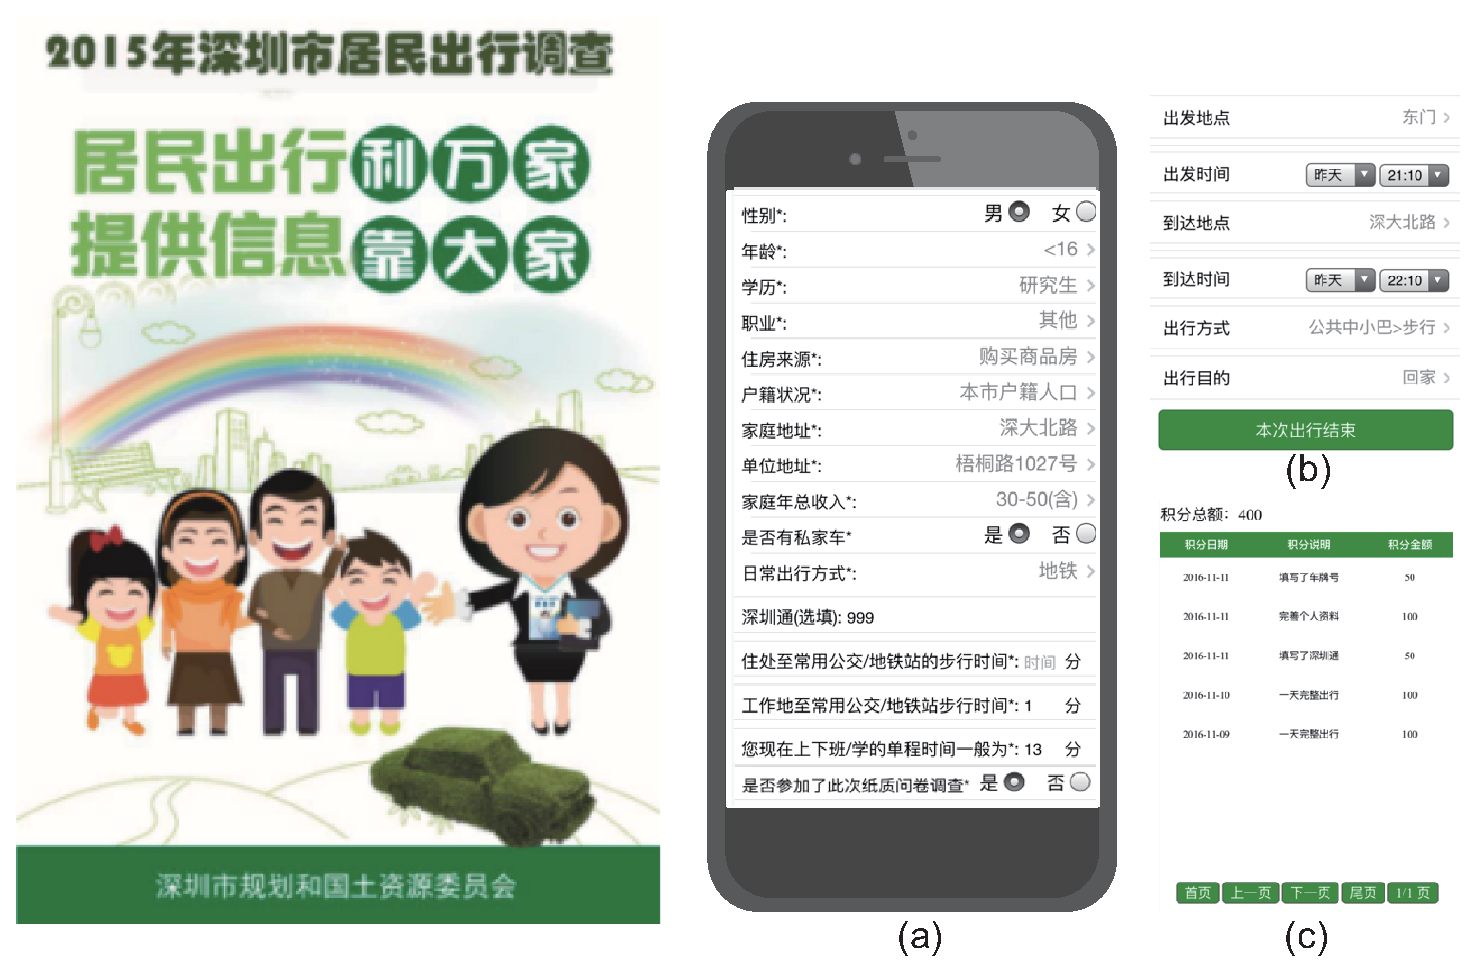
\includegraphics[width=\columnwidth]{pictures/survey_app}
 \caption{Collecting Interface: (a) welcome page; (b) personal characteristics collecting page; (c) trips collecting page; (d) credit system page}
 \label{fig:app}
\end{figure}


Over the releasing time period from June to October in 2015, 25481 individules were reached and XXX trips are collected, XX trips per individual. Figure~\ref{fig:data_over} lists the XX variables, falling into 8 domains. Those domains give a generalized depiction of the individual characteristics and serve as the ingredients for the analysis of urban dynamics over diverse people. 

Considering the caveat that self-selecting individuals are most unlikely to represent any clearly defined population~\cite{Longley2015}, a series of statistical analysis is performed to check whether it is rich enough to represent a wide range of human individuals in the city.


\begin{figure}[htb!]
 \centering % avoid the use of \begin{center}...\end{center} and use \centering instead (more compact)
 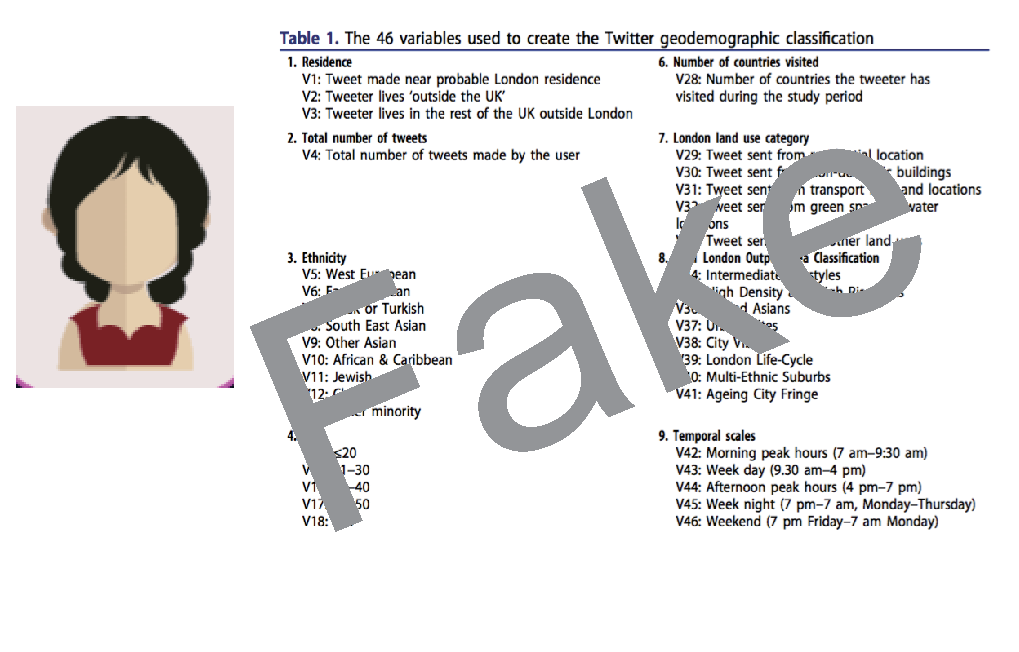
\includegraphics[width=\columnwidth]{pictures/data_over}
 \caption{Profile of Individual: XX variables falling into 8 domains enriches the analysis of urban dynamics}
 \label{fig:data_over}
\end{figure}

According to the 2015 Annual Census Statistics report~\footnote{http://www.sztj.gov.cn/xxgk/tjsj/pcgb/201606/t20160614\_3697000.htm}, people aging 15-64 occupy 83.23\% and the median age is 31.5. Shenzhen is majority of young people. 

\textit{Overview} Figure~\ref{fig:data_stat} shows samples covering almost all ages and age between 18 to 45. The 

\textit{Compared to Census} In the report (looking for some report), the penetration of mobile device is XXX, almost every XX people got a Mobile Phone in the urban. XX.  multiple social characteristics of a people is sampled, including income, education, etc. age and income distribution follows the social architecture. 


\begin{figure}[htb!]
 \centering % avoid the use of \begin{center}...\end{center} and use \centering instead (more compact)
 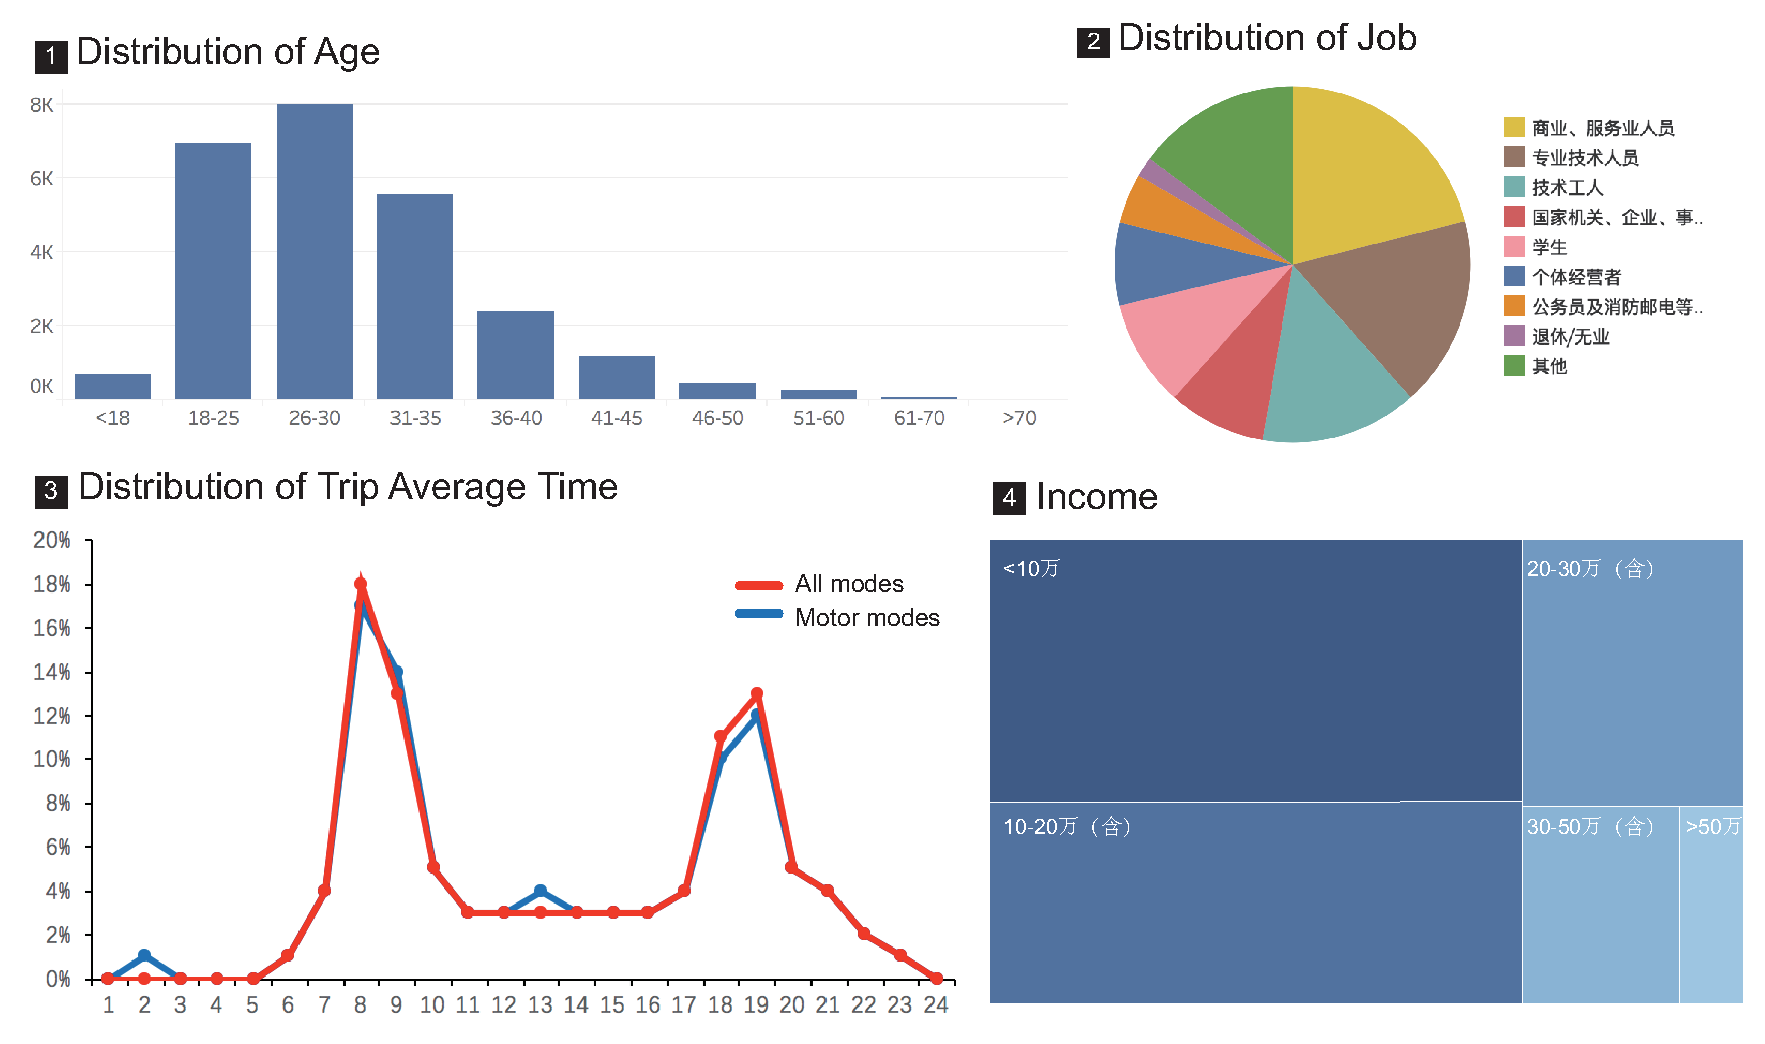
\includegraphics[width=\columnwidth]{pictures/data_detail}
 \caption{Statistical Overview of Social Characteristics}
 \label{fig:data_stat}
\end{figure}



% \section{Overview}

\lmc{Add a paragraph to introduce the motivation of this work, where we derive the tasks via the interview with domain exports.}

The design of the system is driven by tasks, to align the analysis of mobility patterns with individual characteristics. Before diving into the design of the system, we introduce the couple of specifical tasks the system intended for. 

\begin{itemize}
\item \textit{Task 1: Identify the group with specific individual characteristics}: to get groups of people with common or close attributes, to explore the correlation among individual characteristics.
\item \textit{Task 2: Explore the mobility patterns of a group}: to explore where, how and why an interested group go in the city. 
\item \textit{Task 3: Compare mobility patterns among multiple groups}: to know the similarities and differences between different groups in their mobility patterns, to investigate the relationship between movement and individual characteristics.
\end{itemize}

\subsection{Design Considerations}

With these three tasks, we derive following design considerations:

\begin{itemize}
\item \textit{Intuitive perception of an individual as an organic complex (C1)}: the system should make use of users' daily life experience in knowing people to provide intuitive visualization, instead of the lifeless representation by number. The visual design needs to help end-users to pick desirable ones from the mass. 
\item \textit{Good overview of the multivariate individuals (C2)}: following the visual analytics manta by Shneiderman~\cite{RN459}, it is very important to provide a good overview of all the individuals then the users know where to explore. 
\item \textit{Effective multivariable cross-filter for individual characteristics (C3)}: there are eight domains to describe an individual. The system is supposed to provide a straight-forward way for easy filtering by the eight criteria. 
\item \textit{Compact visualization of mobility patterns in the constraint of spatial space (C4)}: the analysis of mobility patterns not only includes the conventional spatial and temporal dimensions, but also other abstract dimensions, e.g., travel purpose, visiting frequency, etc. The system should handle a compact layout to support the easy correlation between spatial and abstract information. 
\item \textit{Flexible interactions to explore the mobility patterns either within one group or between groups (C5)}: to support the comparison among groups, \textit{Task 3}, the system should maintain flexible interactions which allow the end-users to explore freely.
\end{itemize}

% Classification method, flow clustering method, Semantic representation. 

With those design considerations, we develop a visual analytics system as Figure~\ref{fig:teaser} shows. It composes of individual panel (the left part) for individuals (\textit{Task 1}) and spatial panel (the right part) for the mobility pattern (\textit{Task 2 and 3}). In the individual panel, interactive infographics, t-SNE visualization, and data-driven profiles support users to narrow the scope down to groups of individuals with interested characteristics. With the chosen group of individuals, its moving related information is visualized and explored in a 2.5D spatio-temporal view.



\section{System Design}


This work we try to answer following questions:

Problem to solve: 
\begin{itemize}
\item \textit{What flows of people with certain demographic characteristics}: multiple attributes, semantic understanding, loose attribute boundary
\item \textit{What the Urban Dynamics of the Group}: where those people go and how they access the ... in a city. the patterns of behaviour classified by different social characteristics.  Including travel purpose, 
\item \textit{Compare of moving patterns between different groups}: what the similar and difference between groups in their traveling behaviour
\end{itemize}

We derive the design considerations:

\begin{itemize}
\item \textbf{C1: semantic understanding of demographic cahracteristics}: since the concept of groups is vague to define directly quantitativily. The visual design needs to consider how to help end-users to pick desirable ones from the mass. 
\item \textbf{C2: }
\end{itemize}

Classification method, flow clustering method, Semantic representation. 

The key of our work is to align the analysis of urban dynamics with the available of individual characteristics. 

Semantic understanding of social characteristics.

\subsection{Data-driven Profile Visualization}

Glyph-based visualization~\cite{borgo2013glyph} is the form of visual design to compose multivaribles into a collection of unified visual symbols, known as glyph. Glyph is intended for quick understanding and aligned comparison. Among glyph design, Chernoff Face~\cite{chernoff1973use} represents data variabules by the different features of a cartoon face. Following the idea of Chernoff Face~\cite{chernoff1973use}, we design a type of glyph, a graphical representation of people with specific demographic characteristics. The idea behind using faces is that humans easily recognize faces and notice small changes without difficulty. Those visual profiles are intended for intutive visual understanding and clustering, to abstract to concrete and semantic understanding, to help users clues to target the interested individual groups effectively.

Figure~\ref{fig:design_profile} shows the legend for the user profile. Those design dimensions are driven by data.The eight demographic dimensions are systematically designed into different visual symbols. Considering there are two types of variables, i.e., the numeric attributes and categorical attributes. By different composition, stimulus pattern which has the abstract deomgraphic measurement of individuals.

\begin{itemize}
\item \textbf{Gender} the gender is visually mapped to the hair style of the avatar. 
\item \textbf{Age} age is implied by the decoration on the hair. For the elder above 70, the hair is dyed to gray. For the youth beneath 18, hair decoration for girls and boys are adapted to the hair style.
\item \textbf{Education} The thickness of eye glasses is used to indicate the different levels in education.
\item \textbf{Job} The clothes is designed to imply the job of the individual. There are 9 types of clothes.
\item \textbf{Belongings} for house, car, residential license are considered as the belongings to the individual, so we design each of them as an add-on decoration to imply whether the individual has it or not.
\item \textbf{Income} a money symbol is used to show the different income levels.
\end{itemize} 

\begin{figure}[htb!]
 \centering % avoid the use of \begin{center}...\end{center} and use \centering instead (more compact)
 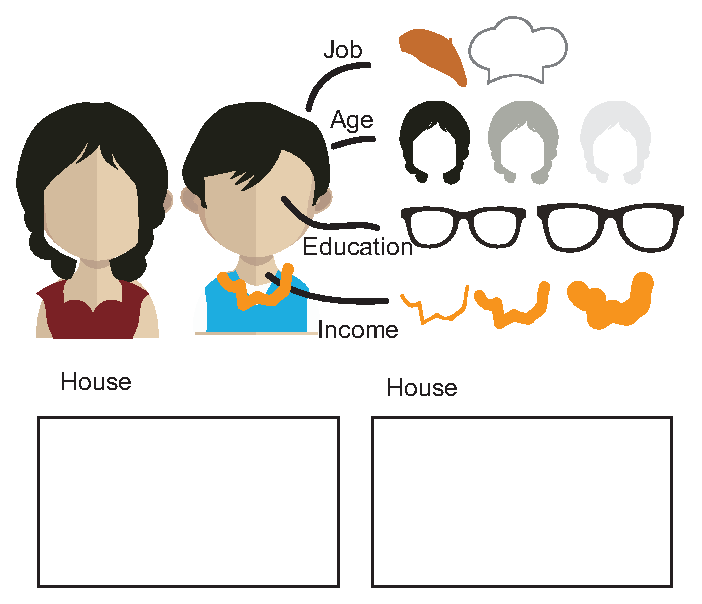
\includegraphics[width=\columnwidth]{pictures/design_profile}
 \caption{Design Profile}
 \label{fig:design_profile}
\end{figure}

With the visual mapping, the profiles varies from individual to individual. Figure~\ref{fig:div_profile} shows some examples. By concretizing the attributes which otherwise is too abstract to percept, users can scan and search for interesting target organically in figures.

\begin{figure}[htb!]
 \centering % avoid the use of \begin{center}...\end{center} and use \centering instead (more compact)
 
\includegraphics[width=\columnwidth]{pictures/design_div}
 \caption{Diverse Profile}
 \label{fig:div_profile}
\end{figure}

\subsection{t-SNE Projection}

Each individual is denoted as a vector with eight factors and projected as a dot into the 2D view via t-SNE project~\cite{maaten2008visualizing}, which well suits high-dimensional data for visualization in a low-dimensional space of two dimensions. As Figure~\ref{fig:tsne}(a)shows, all volunteers are embedded evenly in the 2D view, indicating the uniformly sampling over demographical space. 

Multiple views of abstract view, t-SNE proection and semantic data driven profile visualization are coordinated in a Cross-filter machinesm~\cite{Weaver2010}. It allows end-users to interactive drill-dowm into individuals with interested characteristics from multiple perspectives. Starting from the abstract criterion constraints, the scope of interest is narrowed down to individuals with(out) certian properties. And then further cross-filtering with semantically visual profiles, to check the combination of 8 characteristical variables. Figure~\ref{fig:tsne}(b) examplifies four groups of interest. 

\begin{figure}[htb!]
 \centering % avoid the use of \begin{center}...\end{center} and use \centering instead (more compact)
 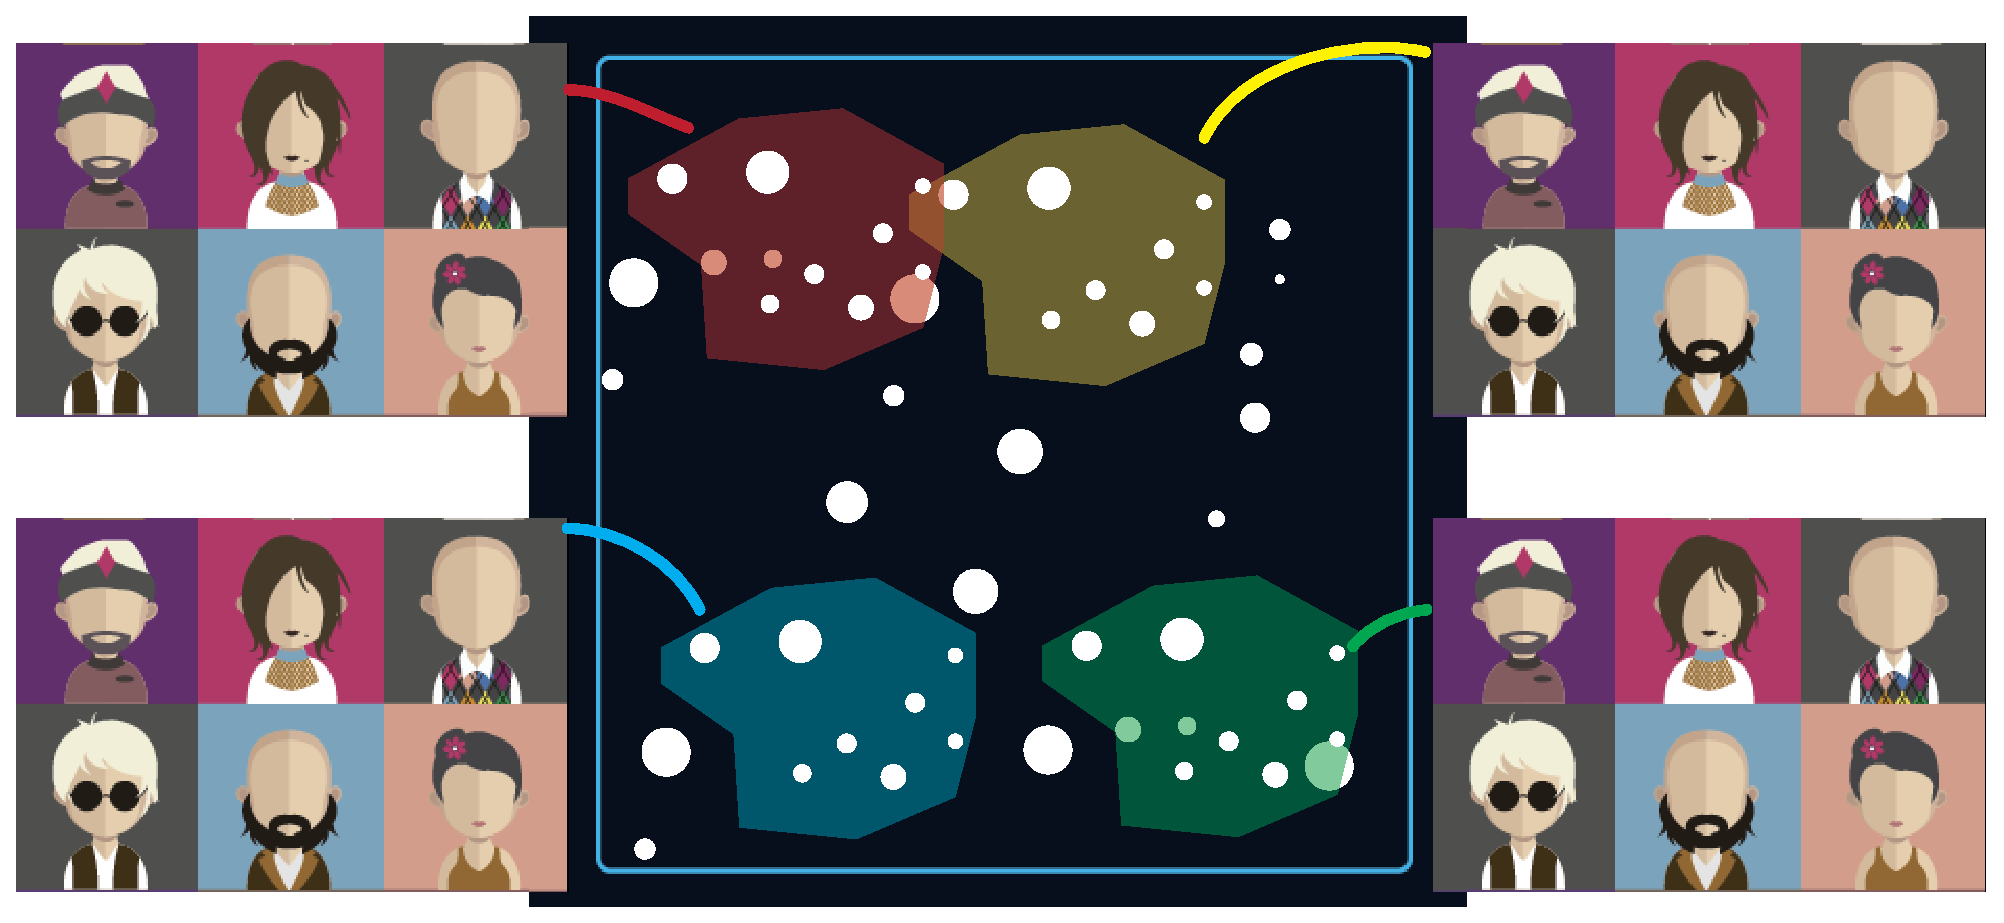
\includegraphics[width=\columnwidth]{pictures/mds}
 \caption{t-SNE project with four groups of the interest}
 \label{fig:tsne}
\end{figure}

\subsection{2.5D Spatial Visualization}

Embedding multiple variables in the spatial map is a challenging problem. Distortion technique 2D spatial, such as the partial route embedding~\cite{sun2016embedding}. However, when it comes to the global visualization, the trade-off between occlusion-free and the spatial perception. Follow the idea of 2.5D space design~\cite{Tominski2012_stacking}, the space visualization is embedded in 2.5D space, which also can smoothly transited back to the conventional 2D view.  

 Each TAZ is grown as a prism whose height encodes the occurrence of visiting. Brunch of TAZ with similar visiting pattern and purpose are grouped by an heuristic DB-Scan Algorithm in the context of TAZ. From a center TAZ, walk to neighbour TAZ to check whether aggregation or not. The aggregated TAZ brunch indicates the region visiting by the group of people in same purpose, which is often the popular traveling places. The TAZ brunch is visualized...

 To compare the mobility patterns across different groups of people, a Small Multiple dock is used to reserve the ever explored interesting result. To simply the comparion over spatial distribution, the snapshot is rendered in the 2D space, which can be magnified to check for the details in the 2.5D space.

 In this view, it supports end-users to direct manipulate the space, e.g., zooming, panning, etc. Also, detail information about the visiting can be checked by direct clicking on the TAZ. 
% \section{Experts Feedback}

\lmc{Add a section to introduce the domain experts' feedback}


\lm{We interview XX domain experts from the GIS field. XX of them are with ... The procedure went as following. We first introduce them the system an...}

\section{Case Study}

Applied the system to Shenzhen's dataset. We demonstrate the efficiency. 

\subsection{OVERVIEW Case 1: City Folding}

compare the distorted maps from various groups

Different different groups of people and see their patterns across the city.

Group 1 is defined as xxxxx. The popular visiting places

Wealthier people with better access to ... than poor people. 

\subsection{DETAIL Case 2: Look into Detail}

check the detail information of a group

To compare the Group 1 and Group 2, the similar places and different places...

\section{Conclusion}
\label{sec:conclusion}

Combined travel demands, this work illustrates the relationship between accessibility and behaviour within the region, which in turn can be used to forecast the traveling trips. 

derive zonal level analysis thich can be used in transportation applications.

Our analysis demonstrates how demographics survey collectd via social media have the potential to indiate the movement patterns of groups that have different social charactersitics and the difference in using urban facilities. Better understand of the interactions between population characteristics and their urban activity. The data we used represent a small propotion of the population of which we do not have the clear definition of its demographics. We consider this work as one of the first steps of research contextualize the analysis of urban dynamcis with social science, to understand the  interactions between population characteristics and their urban activity. 

\bibliographystyle{abbrv}
%%use following if all content of bibtex file should be shown
%\nocite{*}
\bibliography{main}
\end{document}
